%\subsection{Specific Aim 2: Functional Materials}
\subsection{Specific Aim 2: Hydrodynamics and ...}
\label{subsec:specific_aim_2}
Specific Aim 1 dealt with the collective material property of amphiphiles which does not involve the movement  of the solvent.
In Specific Aim 2, we include hydrodynamics effects. The reason for including hydrodynamic effects is that 
biologically relevant functions like fusion, fission, pore dynamics involve viscous dissipation of the aqueous environment. 
Moreover, including hydrodynamics adds relevance to our theory since most coarse-grained and molecular dynamics theories
include water either explicitly or implicitly in their models. 


%The mathematics of this proposal investigates how three-dimensional solids deform under long-range surface tension interaction. The results generalize the physical principles used in the design of functional materials, enabling investigators to simulate sub-micron scale systems that are otherwise impractical to realize experimentally. It supplies new insight into organizational principles in physical and biological sciences. 
%
Over the past decade, there has been an explosion of interest in the fabrication of complex microscopic three-dimensional structures 
\cite{Cho2010}. These fabrication processes utilize the fact that at small scales, capillary forces dominate  van der Waals interactions and thermal noise  \cite{Zhang2017}, enabling the coordinated movement and binding of material subunits. Two prominent fabrication techniques are capillary origami 
\cite{Pandey2011,Leong2007,Reynolds2019} and colloidal self-assembly \cite{Dasgupta2017,Siontorou2017}. Capillary origami uses principles of elastocapilirity wherein elastic solids deform under surface tension \cite{Bico2018,VanHonschoten2010}. In self-assembly of colloids, 
particles exhibit similar thermodynamic behavior of molecular systems, except that the behavior occurs over observable, long time scales \cite{Zhang2017}. 

There is inherent intellectual value in fabricating novel three dimensional structures: Living cells construct biological molecules like proteins, membranes and viral capsids using hierarchical assembly \cite{Whitesides2002}. At the same time, elastocapillarity and colloidal self-assembly supply model systems for biological processes, like vesicle adhesion and membrane bound protein interaction \cite{Dasgupta2017}, the hydro-polar model of protein folding \cite{Lau1989,Pandey2011} and viral capsid assembly and \cite{CASPAR1962}. Capillarity can serve as a model for the lock and key mechanism binding between the active site of an enzyme and a substrate molecule \cite{Araujo2018}, or treating viruses like adhered particles 
\cite{Agudo-Canalejo2017,Agudo-Canalejo2015,Deserno2004}, or studying decorated vesicles 
\cite{Auth2009,Weikl2002,Atilgan2007}. Although challenging, mathematically analyzing these model systems gives deep insight into biological structure and function.

%Aside from their intellectual value, high-yield batch production of three-dimensional microstructures has application in functional materials engineering \cite{Syms2003,Leong2010,Crane2013}. In mechanics, for instance, elasticapillarity is a guiding principle lithographic etching of electronics \cite{Bico2018}. Researchers have used self-folding structures in the design of micro containers for encapsulated drug delivery \cite{Fernandes2012} and 3D photovoltaic cells \cite{Guo2009}. 
%In chemical engineering, emulsions stabilize droplets through capillary binding or particulates leading 
%to colloidosomes capturing proteins, vitamins, flavors, living cells \cite{Dinsmore2002}. 
%Microsensors, electronic ink and micromotors \cite{Zhang2017,Yan2016} 
%are potential applications involving Janus-like particles. 

\begin{wrapfigure}[14]{r}{3.0in}
\vspace*{+15pt}
\centerline{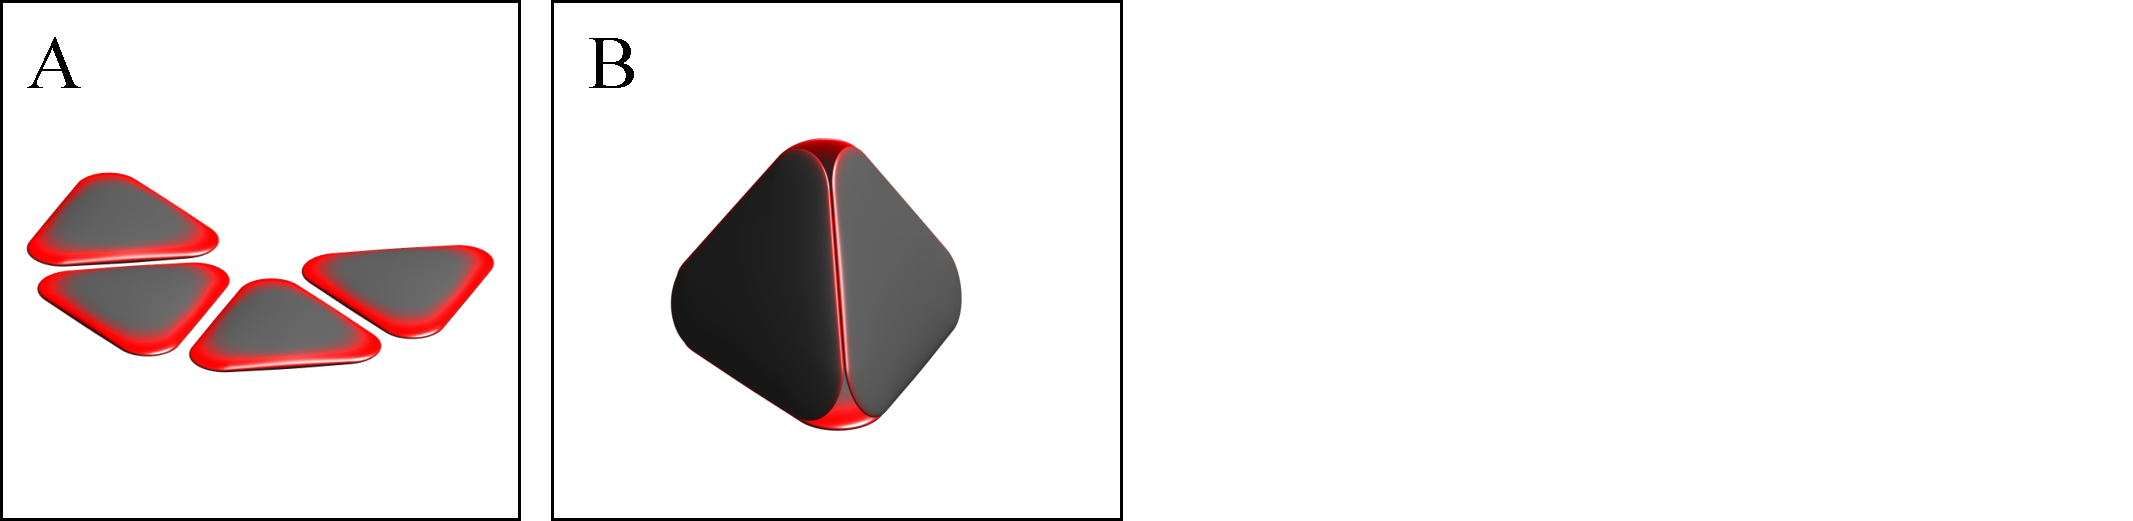
\includegraphics[width=3.0in]{figures/SA3_fig2.pdf}}
\vspace*{5pt}
\caption{{\footnotesize Illustration of self-assembly of hydrophobically labeled faces.
The thick triangles have a rim-hydrophobic label on one side, and are hydrophilic on the other side.
These shapes would potentially aggregate into a tetrahedral container. }}
\label{fig:illustration}
\end{wrapfigure}
The HAP theory is ideally suited to the problem of creating microstructures through capillary action. Specifically, the modeling application considers the assembly of polyhedra from smaller subunits. Our developments, which include viscous interactions, thermal fluctuation, and a long range description of capillarity, will pave the way for dynamical understanding to organizational principles in viral capsid formation, for instance \cite{CASPAR1962,Prasad2012}. 

In order to illustrate the novelty of our approach, it is helpful to first describe how current experimental and mathematical techniques deal with polyhedral assembly. Capillary origami uses lithography to etch faces out of a thin, elastic sheet \cite{Pandey2011,Reynolds2019}. The collection of faces form a so-called net, and this net self-folds into a three-dimensional polyhedron (Figure~\ref{fig:illustration}). The motivation is to create micro containers to mimc protein folding \cite{Reynolds2019}. Prediction of geometric structure from its subunits is non-trivial. That is because the final morphology depends on the net structure, physical interactions, and the surrounding media, and researchers have formulated optimality criteria for these nets \cite{Araujo2018,Pandey2011}. 

The experimental shapes are hundreds of microns in diameter. Thus, as a key distinction with HAP approach, the driving force for folding in capillary origami and related processes comes from surface energy of the hinges (e.g. soldered hinges that supply a surface tension once the system is heated). Mathematicians have numerically and analytically described the behavior of these surface tension driven hinges \cite{Bico2018,Peraud2014,Brubaker2016}, making it possible to simulate the mechanical problem, in principle, using slender body theory for plates. 

To study this problem using HAP theory, we form a collection of thin, prism-like particles in Figure \ref{fig:illustration}. 
Each of these particles serves as a face in the final morphology. The edges of the prisms are labeled hydrophobic according to the boundary condition in the screened Laplace equation boundary value problem. This way, the edges coalesce, forming the desired structures. Furthermore, 
by manipulating the boundary condition in HAP, it is possible to have faces attach and detach with precision, and form a net or other structures if so desired. Our HAP theory therefore generalizes submillimeter theoretical and experimental work to the micron and nanometer sizes. 

%There is also the possibility to explore new classes of mathematical materials, like wrinkling in polystyrene sheets \cite{Paulsen2016}, that include the interaction between an elastic material, the viscous solvent, and long range hydrophobic (capillary) interactions. In the case of rigid particles and subunits, the rigid body motions come from the so-called mobility boundary value problem for the Stokes equation. Here, the hydrophobic stress balances with the viscous stress coming from the rigid body motion of the particles in the surrounding solvent. If the particles are deformable, like a protein \cite{Elms2012} or as in the capillary induced bending of rods \cite{Schulman2017}, then we can formulate an elastic energy for deformation. These elastic energies account for surface bending or even permanent charge. To deploy this approach, it is a matter of solving the bodies' momentum balance equations coupled to the fluid through the viscous, elastic, and hydrophobic stress balance. 

\begin{figure}
\begin{center}
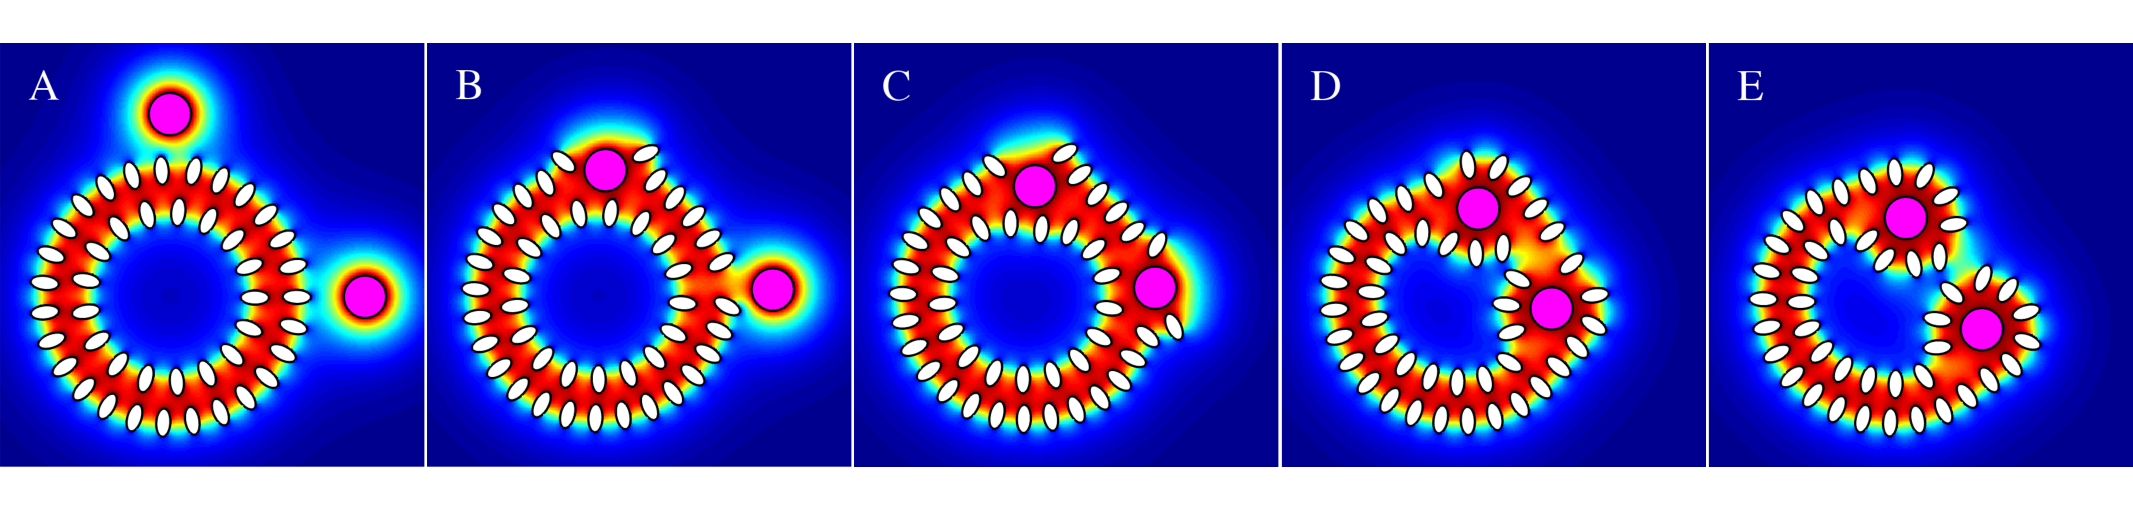
\includegraphics[width=\textwidth]{figures/SA3_fig1.pdf}
\end{center}
\caption{(A)--(D) shows the spontaneous insertion of two hydrophobic particles into a vesicle bilayer. 
The driving force is long-range interaction between the hydrophobic, magenta particles and
the bilayer core.  The particle entrainment cause the vesicle to break apart, analogously to surfactant
induced lysis.}
\end{figure}
Finally, further applications of our modeling approach include colloidal interaction on interfaces. Here, the experimental setups use Janus particles to model, for example, membrane bound proteins \cite{Kumar2013,Lehle2008,Zhang2017}. The idea of an amphiphilic Janus particle was introduced by P. G. de Gennes in 1991 \cite{Zhang2017}. The Investigators have significant experience as Janus particles figure heavily into our particle based description of bilayers, and can adjust our modeling approach to account for proteins. This is done by consider mixtures, consisting of many (hundreds to thousands) long, elongated amphiphilic particles for the lipid phase. Larger particles with hydrophobic patches or stripes model the proteins \cite{Jurasek2017}.

The distinction between macroscopic capillarity and microscopic hydrophobic force are relevant here as well.  Prior models use surface energies to account for interaction between particles in an interface \cite{Dasgupta2017}. 
However, this may be missing important physics, and here our modeling approach has the advantage in that protein insertion, for instance, is a self-consistent consequence of the formulation, versus an assumption imposed by boundary conditions.  
The simulations will enable us address important biological questions on how a collection of 
interface bound colloids interact \cite{Yao2013,Salib2013}, 
and how configurations dictate 
macroscopic surface properties and sense background curvature \cite{Cavallaro2011,Liu2018,Sharifi-Mood2015}. 

